\documentclass[12pt]{report}
\usepackage{amsmath,amsthm,amssymb,amsfonts,setspace,graphicx,subfigure,verbatim}
\usepackage{adjustbox}

\usepackage{adjustbox}

\usepackage{listings}
\usepackage[italian]{babel}
\usepackage[a4paper, portrait, margin=0.85in]{geometry}

\usepackage[colorlinks]{hyperref}


\begin{document}
\title{Vehicular communications}
\author{Ollari Ischimji Dmitri}

\maketitle

\newpage

\tableofcontents
\listoffigures
\listoftables

\chapter{Introduction to Vehicular Communications}
\section{Principles and challenges}
\section{Standardization and open issues}
\section{ITS Architecture}
\section{ITS Applications}
\section{Autonomous driving}

\chapter{Telecomunicacion network basics}
\section{The OSI and Internet models}
\section{Communication models}
\section{Delimitation}
\section{Sequence control}
\section{Error management}

Il controllo dell'errore ha 3 possibili soluzioni:
\begin{itemize}
	\item \textbf{Error detection}: rilevazione dell'errore
	\item \textbf{Error correction}: correzione dell'errore
	\item \textbf{Error recovery}: recupero dell'errore
\end{itemize}

%TODO: skippato da pagine 61, DA FARE
% WARN: PARTO DA PAGINE 69
%WARN: finire da pagina 79

\subsection{Complement sum}

\begin{figure}[!ht]
	\centering
	% TODO: ingrandire immagine a 0.4
	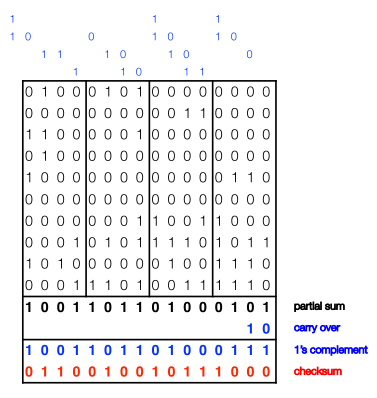
\includegraphics[width=0.3\columnwidth]{./images/complement_sum.png}
	\caption{Complement sum}
	\label{fig:complement_sum}
\end{figure}

Quando si riceve il pacchetto, si calcola il \textbf{checksum} dei dati ricevuti(come in \autoref{fig:complement_sum})
e lo si confronta al checksum allegato al pacchetto ricevuto,
nel caso di checksum differente si deve ritrasmettere il pacchetto.

\subsubsection{Other codes}

\textbf{Polynomial codes} conosciuti anche come \textbf{Cyclic Redundancy Check(CRC)},
usano moltiplicazioni tra polinomi per effettuare il checksum.

\subsection{Error correction}
Con la \textbf{block parity check} si possono recuperare errori ma solo se presente un errore di 1 bit.

Vengono quindi introdotte tecniche \textbf{Forward Error Correction(FED)}(\href{https://en.wikipedia.org/wiki/Viterbi_algorithm}{ad esempio Algoritmo di Viterbi})
che permettono di capire la presenza di un errore mediante algoritmi di ricostruzione.

Con FED si ricorre a ridondanza per eliminare errori(pochi in numero), non sono necessari messaggi
di corretta ricezione, che torna molto utile nel caso di comunicazione unidirezionale.


\begin{figure}[!ht]
	\centering
	% TODO: ingrandire immagine a 0.4
	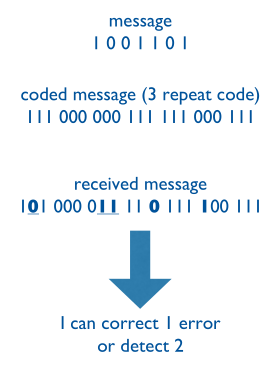
\includegraphics[width=0.3\columnwidth]{./images/repetition_code.png}
	\caption{Repetition code}
	\label{fig_repetition_code}
\end{figure}

\section{Error recovery}

Quando si parla di comunicazione in reti di comunicazioni, si ricade nel richiedere automaticamente
un pacchetto che non risulta corretto al ricevitori,
esistono approcci automatici come \textbf{Automatic Repeat Request, ARQ}.

Esistono inoltre differenti meccanismi di ritrasmissione che come punto focale hanno:
\begin{itemize}
	\item Error detection
	\item Acknowledgements
	\item timers
	\item IU identifiers
\end{itemize}


Le procedure ARQ cambiano in base alla dimensione delle finestra:
\begin{itemize}
	\item \textbf{Stop and wait}: finestra di dimensione 1, si attende l'ack prima di inviare il pacchetto successivo
	\item \textbf{Sliding window, go-back-N}: finestra di dimensione N, si inviano N pacchetti prima di attendere l'ack(non ha un selettore per il resending e invia tutto il blocco)
	\item \textbf{Sliding window, selective repeat}: finestra di dimensione N, si inviano N pacchetti prima di attendere l'ack(ha un selettore per il resending e invia solo il pacchetto corrotto)
\end{itemize}


\subsubsection{Stop and Wait}

Il pacchetto \textbf{ACK(acknowledgement)} solitamente è molto corto per evitare
correzzioni nel pacchetto che conferma la corretta ricezione.

È necessario stabilire un tempo limite entro il quale si da per scontato
la \textit{scomparsa} del pacchetto, solitamente si basa sul \textbf{Round Trip Time(RTT)} che
dipende dalla congestione  della rete e ne misura i ritardi per arrivare da punto A a punto B.

Altro fattore chiave è capire quali dati sono stati inviati e quali no, per evitare
duplicazioni.
Per questo problema di è scelto di indicizzare i pacchetti con una sequenza che prende
il nome di \textbf{SeQuence Number(SQN)} per identificare univocamente quali pacchetti da ritrasmettere.

Si può parlare anche di ACK comulativi mediante l'uso di SQN consecutivi.

\begin{figure}[!ht]
	\centering
	% TODO: ingrandire immagine a 0.4
	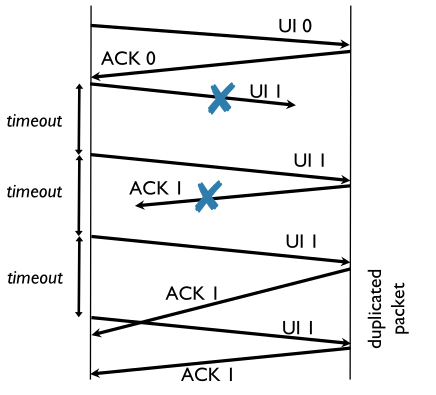
\includegraphics[width=0.3\columnwidth]{./images/esempio_comunicazione_stop_wait_no_sqn.png}
	\caption{Esempio comunicazione stop and wait senza SQN}
	\label{fig:esempio_comunicazione_stop_wait_no_sqn}
\end{figure}


\begin{figure}[!ht]
	\centering
	% TODO: ingrandire immagine a 0.4
	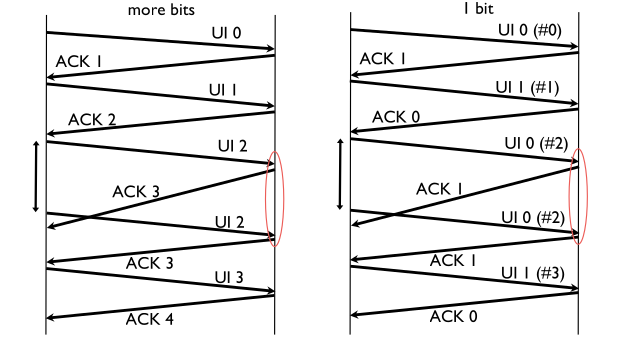
\includegraphics[width=0.3\columnwidth]{./images/esempio_comunicazione_stop_wait_sqn.png}
	\caption{Esempio comunicazione stop and wait con SQN}
	\label{fig:esempio_comunicazione_stop_wait_sqn}
\end{figure}



\subsubsection{Stop and wait performance}

I tempi considerati sono:
\begin{itemize}
	\item \textbf{$T_U$}: tempo di trasmissione di un pacchetto, misurato in $s/IU$
	\item \textbf{$T_P$}: tempo di propagazione di un pacchetto, misurato in $s/IU$
	\item \textbf{$T_{A}$}: tempo di trasmissione di un ACK, misurato in $s/IU$
\end{itemize}

Il tempo totale per inviare un'unità informativa(caso ideale):
\begin{align}
	T_{tot} = T_{U} + 2T_{P} + T_{A}
\end{align}

Il massimo grado di utilizzo di un canale di comunicazione nel caso di \textbf{assenza di errore}:
\begin{align}
	\rho_0
	 & =\frac{T_U}{T_{tot}}                                         \\
	 & = \frac{T_U}{T_U + 2T_P + T_A}                               \\
	 & = \begin{cases}
     \frac{1}{2 + 2 \frac{T_P}{T_U}} \quad \text{se}\quad T_U = T_A  \\
		     \frac{1}{2 \frac{T_P}{T_U} + 1} \quad \text{se}\quad T_U >> T_A \\
		     0 \quad \text{se}\quad T_P >> T_U
	     \end{cases}
\end{align}



Nel caso di \textbf{presenza di errore}, non viene ricevuto l'ACK dal trasmettitore, devo fare alcune assunzioni:
\begin{itemize}
  \item Indipendenza statisticamente dei pacchetti informativi
  \item perdita di pacchetti ACK
\end{itemize}

Indico con $p$ la probabilità di perdita del pacchetto.
%WARN: finire da pagina 79




%  TODO: arrivato a pagina 82
% TODO: prof arrivato almeno a pagina 85


\chapter{Intra-vehicle Communications}

\section{Bus Systems}

\subsection{Perchè usare i bus?}
Un bus che collega tutti i componenti al posto di avere una topologia a grafo completo ha i seguenti vantaggi:
\begin{itemize}
	\item \textbf{Riduzione dei costi}: meno cavi e meno connettori
	\item \textbf{Riduzione del peso}: meno cavi
	\item \textbf{Riduzione del volume}: meno cavi
	\item \textbf{Alta modularità}: modifica veicoli
	\item \textbf{Alta modularità}: cooperazione con OEM
	\item \textbf{Modularità}: riuso di moduli
	\item \textbf{Standardizzazione}: standardizzazione dei componenti e dei protocolli (meno errori scemi)
\end{itemize}




\subsection{Casi d'uso per intra-vehicle communications}

\begin{itemize}
	\item Driveline: Engine and transmission control
	\item Active Safety: Electronic Stability Programme (ESP)
	\item Passive Safety: Air bag, belt tensioners
	\item Comfort: Interior lighting, A/C automation
	\item Multimedia and Telematics: Navigation system, CD changer
\end{itemize}

La geolacaliuazione è fornita da protocolli di navigazione satellitare. I più famosi sono:
\begin{itemize}
	\item GPS: USA
	\item Galileo: EU
	\item Glonass: Russia
	\item Beidou: China
\end{itemize}

Altre soluzioni sono RTK(Real Time Kinematic)!!



\subsection{Classificazione: On-board-communcation}
\begin{itemize}
	\item Complex control and monitoring tasks: trasmissione dei dati tra ECUs(Engine Control Unit) e MMI(Man Machine Interface simile a HMI che sta per human machine interface)
	\item Simplification of wiring: rimpiazzare i fili di rame con bus per ridurre la complessità dei cablaggi
	\item Multimedia bus systems: Trasmette un sacco di dati per i sistemi di intrattenimento
\end{itemize}


\subsection{Classificazione: Off-board-communication(OBD connector)}
\begin{itemize}
	\item Diagnostics: diagnosi del veicolo
	\item Flashing: aggiornamento del software
	\item Debugging: debug del software
\end{itemize}

\subsection{Classificazione per casi d'uso e importanza}

\begin{table}[!ht]
	\begin{adjustbox}{width=\columnwidth,center}
		\begin{tabular}{|c|c|c|c|c|c|c|}
			\hline
			Application            & Message Length & Message rate & Data rate & Latency & Robustness & Cost \\
			\hline
			Control and monitoring &                & 2            & 2         & 3       & 3          & 2    \\
			\hline
			Simplified wiring      &                &              &           & 1       & 2          & 1    \\
			\hline
			Multimedia             & 1              & 2            & 3         & 1       & 1          & 3    \\
			\hline
			Diagnosis              &                &              &           &         &            & 1    \\
			\hline
			Flashing               & 2              &              & 2         &         & 1          &      \\
			\hline
			Debugging              &                & 1            & 1         & 2       &            &      \\
			\hline
		\end{tabular}
	\end{adjustbox}
	\caption{Classificazione per casi d'uso e importanza}
	\label{tab:classification_use_case}
\end{table}


\subsection{Classificazione SAE(Society of Automotive Engineers)}

\begin{table}
	\begin{adjustbox}{width=\columnwidth, center}
		\begin{tabular}{|c|c|c|c|}
			\hline
			Class & Data rate  & vantaggio                    & Dispositivi     \\
			\hline
			A     & $10kBit/s$ & Economico                    & Diagnosi        \\
			B     & $64kBit/s$ & Correzione errori            & Networking ECUs \\
			C     & $1MBit/s$  & Comunicazione in tempo reale & Drive train     \\
			D     & $10MBit/s$ & Bassa latenza                & X-By-Wire       \\
			\hline
		\end{tabular}
	\end{adjustbox}
	\caption{Classificazione SAE}
	\label{tab:classification_sae}
\end{table}



\subsection{Network Topologies}

\begin{itemize}
	\item \textbf{Repeter}: amplificazione del segnale a livello fisico
	\item \textbf{Bridge}: medium/timing adaptation, unfiltered forwarding a livello data link
	\item \textbf{Router}: medium/timing adaptation, filtered forwarding a livello network
	\item \textbf{Gateway}: medium/timing adaptation, filtered forwarding, protocol translation a livello application
\end{itemize}


\subsubsection{Wired OR}

\begin{figure}[!ht]
  \begin{adjustbox}{width=0.5\columnwidth, center}
    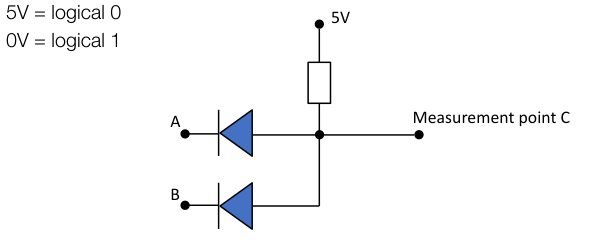
\includegraphics{images/wired_or.png}
  \end{adjustbox}
  \caption{Wired OR}
  \label{fig:wired_or}
\end{figure}

\subsubsection{Wired AND}

\begin{figure}[!ht]
  \begin{adjustbox}{width=0.5\columnwidth, center}
    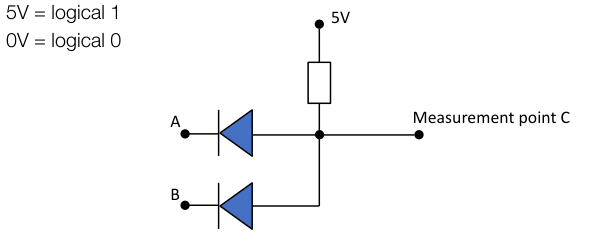
\includegraphics{images/wired_and.png}
  \end{adjustbox}
  \caption{Wired AND}
  \label{fig:wired_and}
\end{figure}


\subsubsection{Wave Effect}
Ad alte velocità entrano in gioco degli effetti non volueti a causa dell'alta velocità.

\begin{align}
  c_0 &= 3 \cdot 10^8 \frac{m}{s}
  \label{eq:velocita_luce}
\end{align}

\begin{align}
  c &\approx \frac{1}{3} c_0 = 10^8 \frac{m}{s}
  \label{eq:velocita_segale_bus}
\end{align}

Il segnale nei veicoli ha un delay di circa $200ns$ quindi il problema insorge quando il tempo per bit è:
\begin{align}
  t_{bit} < 2000ns = 2 \mu s
\end{align}


\section{Bit coding}
\begin{figure}[!ht]
  \begin{adjustbox}{width=0.5\columnwidth, center}
    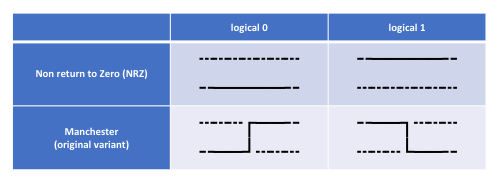
\includegraphics{images/bit_coding.png}
  \end{adjustbox}
  \caption{Bit coding}
  \label{fig:bit_coding}
\end{figure}

Esistono due tipologie di encoding dell'informazione:
\begin{itemize}
  \item Non Return to Zero (NRZ)
  \item Manchester
\end{itemize}

Nella tipologia \textbf{NRZ} il valore logico $0$ è caratterizzato da un segnale basso, mentre il segnale logico $1$ è identificato da un segnale alto.

Nell'encoding di tipo \textbf{Manchester} si pone attenzione al cambio di livello per attribuire il valore logico, il valore logico $0$ è identificato dal passaggio da basso livello ad alto livello e il valore logico $1$ è identificato dal passaggio di stato da alto livello a basso livello.



\subsection{Reducing ElectroMagnetic Interference(EMI)}

\begin{itemize}
  \item Aggiungere schermatura ai fili
  \item usare fili twistati per coppie di fili(annullano effetti di elettromagnetismo a vicenda)
  \item Ridurre la ripidità del segnale
  \item usare usare NRZ che ha pochi cambi di stato
\end{itemize}

\subsection{Clock drift}

Il clock drift è causato dalla costruzione fisica del quarzo usato per il clock, che diffferensce leggermente da altri clock, questo fenomeno causa \textbf{desincronizzazione}.
\subsection{Bit stuffing}
Il problema associato all'utilizzo della codifica NRZ è che inviando una serie di bit costanti, in presenza di piccoli ritardi, i dati vengono ricevuti in maniera sbagliata.

Una soluzione proposta è quella del \textbf{Bit Stuffing} ed inserisce un bit extra dopo $n$ bit consecutivi.
\begin{itemize}
  \item Se ci sono 3 uni di fila, agiunge uno zero
  \item se ci sono 3 zeri di fila, aggiunge un uno
\end{itemize}


\section{Classification according to bus access}

\begin{figure}[!ht]
  \centering
  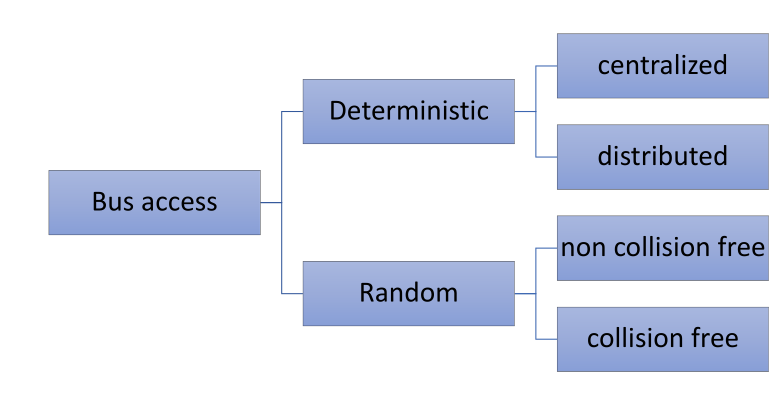
\includegraphics[width=0.4\textwidth]{./images/classification_bus_access.png}
  \caption{Classification according to bus access}
  \label{fig:classification_bus_access}
\end{figure}

\subsection{Deterministic}
\subsubsection{Centralized}
Accesso al bas di tipo \textbf{master-slave}(similare ad un sistema pooling)
\subsubsection{Decentralized}

Protocolli basati su \textbf{token}, tutti collegati a cerchio e si invia il messaggio con un token (che è tipo il bastone della parola) al ricevitore, il ricevitore manda il suo messaggio dopo nella catena insieme altoken e cosi via.

Solo il nodo con il token poò inviare il suo pacchetto di informazioni.


L'altro approccio è il \textbf{TDMA}(Time-division multiple access), si identificano i client attaccati al mezzo di comunicazione e si divide la comunicazioni a slot temporali e si può capire chi invia guardando il riferimento al clock

Grande problema di TDMA è la sincronizzazione.


\subsection{Random}
\subsubsection{Non Collision Free}
\textbf{CSMA/CA(Carrier Sense Multiple Access)/(Collision Avoidance)} misura l'energia del bus e invia quando l'energia è sotto un certo \textit{livello di riferimento}.

CSMA senza CA, se sente il canale occupato, seleziona un tempo random che chiama backoff e aspetta, dopo di che riprova ad ascolare il bus.

CSMA con CA ogni nodo conta il tempo che il noda che sta comunicando finisca, i nodi posso comunicare in qualsiasi momento e quindi ogni conteggio sarà diverso, dopo che il nodo ha finito di comunicare, ogni nodo aspetta il tempo che ha contato il precedenza.

se mentre i nodi stanno aspettando il tempo contato per trasmettere uno dei nodi finisce, si salva il tempo avanzato agli altri nodi e si utilizza quello per il prossimo check di chi tocca.

Questo sistema non è \textit{giusto} e può portare pacchetti a rimanere nella coda per tempi lunghi.



% TODO: descrivere meglio CSMA/CA

\textbf{CSMA/CD(Carrier Sense Multiple Access)/(Collision Detection)} se più nodi comunicano l'energia sul bus è maggiore del solito e i nodi si rendono conto del problema.

I nodi si fermano(per risparmiare risorse) e mandano un segnale \textbf{jamming} che è una sequenza di bit di alto livello per comunicare agli altri nodi il problema e di non comuniicare per un po.

Si applicano ai nodi dei tempi di backoff mediante strategie di backoff e si riprova.

\textbf{CSMA/CR(Carrier Sense Multiple Access)/(Collision Resolution)}:
\begin{enumerate}
  \item \textbf{Arbitration phase}: si compete per avere il canale
  \item \textbf{data}: il nodo che ha vinto il canale comunica
\end{enumerate}

E si itera questo processo ogni volta che un nodo vuole comunicare.


\subsection{Typical structure of an ECU}
\begin{figure}[!ht]
  \centering
  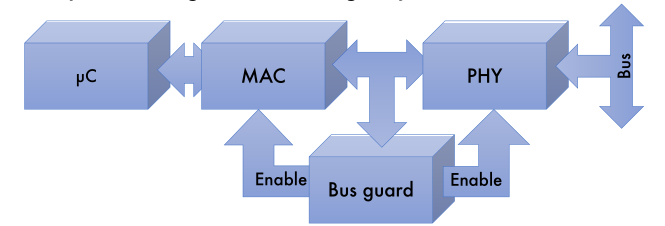
\includegraphics[width=0.4\textwidth]{./images/ecu.png}
  \caption{Struttura ECU}
  \label{fir:struttura_ecu}
\end{figure}





\section{Protocols}


\subsection{Il Bus K-Line}

Il Bus K-Line è un protocollo standard dell'industria degli anni '80, successivamente standardizzato come ISO 9141. Esistono numerose varianti del protocollo, soprattutto a livello di Link Layer. Tuttavia, ci concentriamo principalmente sull'ISO 14230, noto come KWP 2000 (Keyword Protocol), che specifica i dettagli dei livelli fisici e di collegamento. Questo bus è bidirezionale e consente la comunicazione su un singolo filo, noto come la "linea K".

Facoltativamente, può essere presente anche una "linea L" unidirezionale, che consente reti miste. Il Bus K-Line è principalmente utilizzato per collegare unità di controllo elettroniche (ECU) a strumenti diagnostici (tester), anche se è possibile utilizzarlo per la comunicazione diretta tra ECU in casi rari. I livelli logici sono relativi alla tensione a bordo del veicolo, con valori inferiori al $20\%$ che rappresentano "0" e valori superiori all'$80\%$ che rappresentano "1". La trasmissione di bit segue uno schema compatibile con UART (Universal Asynchronous Receiver Transmitter), comprensivo di un bit di start, otto bit di dati, un bit di stop e un bit di parità opzionale. La velocità di trasmissione dei bit può variare da 1,2 kBit/s a 10,4 kBit/s, ma è determinata dall'ECU, non dal bus. Di conseguenza, il master deve essere in grado di gestire più velocità di bit.

\subsubsection{Protocollo del Bus K-Line}

Il protocollo del Bus K-Line prevede una procedura di stabilimento della connessione che esiste in due varianti: "5 Baud init" e "Fast init". Nella prima variante, il master invia l'indirizzo di destinazione utilizzando una velocità di 5 bit al secondo. L'ECU risponde con il valore 0x55 (01010101), che rappresenta il byte basso della chiave di comunicazione, e il byte alto con la velocità di dati desiderata. Il master deduce la velocità di bit dal modello e invia un bit di "Echo" corrispondente all'alto byte invertito. L'ECU risponde con un altro bit di "Echo" corrispondente all'indirizzo di destinazione invertito.

La seconda variante, "Fast init", ha una procedura più rapida (100 ms) e una velocità di bit costante di 10,4 kBit/s. In questa variante, il master invia un modello di "sveglia" (25 ms basso, 25 ms di pausa) seguito da una richiesta di "Start Communication" che include l'indirizzo di destinazione. L'ECU risponde con una "chiave" entro un massimo di 50 ms, la quale codifica le varianti di protocollo supportate.

La comunicazione sul Bus K-Line è sempre inizializzata dal master, che invia una richiesta a cui l'ECU risponde con una risposta. L'indirizzamento può essere a livello fisico (per identificare specifiche ECU) o a livello funzionale (per identificare classi di ECU come motore, trasmissione, ecc.). La durata di una singola trasmissione a 10,4 kBit/s varia da 250 ms nel miglior caso a 5,5 s nel caso peggiore, il che implica un tasso di dati di livello di applicazione inferiore a 1 KB/s.

\subsubsection{Intestazione del Protocollo del Bus K-Line}

L'intestazione di un messaggio K-Line comprende un "byte di formato" che codifica la presenza e il significato dei byte di indirizzo. Inoltre, la lunghezza del pacchetto può essere codificata nel byte di formato, consentendo di omettere il byte di lunghezza. L'intestazione include l'indirizzo di destinazione, l'indirizzo di origine, la lunghezza del messaggio e il payload, che può contenere fino a 255 byte. Il primo byte del payload rappresenta l'Identificatore del Servizio (SID), seguito da un byte di checksum che è la somma di tutti i byte del messaggio, calcolata in modulo 256.

\subsubsection{Service Identifiers (SIDs) del Bus K-Line}

Il Bus K-Line utilizza Service Identifiers (SIDs) per definire il tipo di servizio richiesto o fornito. Tra i SIDs standard troviamo quelli per l'inizializzazione e la terminazione della sessione, come "0x81h Start Communication Service Request" e "0x82h Stop Communication Service Request". Altri SIDs possono essere definiti dai produttori e passati invariati al livello di applicazione. Inoltre, è comune utilizzare due SIDs per ciascun tipo di messaggio: il primo SID rappresenta una risposta positiva, mentre il secondo indica una risposta negativa.

\subsubsection{Gestione degli Errori del Bus K-Line}

La gestione degli errori sul Bus K-Line prevede che, se arriva un segnale errato, l'ECU ignora il messaggio. Il master, d'altro canto, rileva la mancanza di un'accettazione e ripete il messaggio. Se dati non validi vengono inviati, il livello di applicazione può rispondere con una risposta negativa. In questo modo, sia il master che l'ECU possono reagire in modo appropriato agli errori.

\subsubsection{Utilizzo nella Diagnostica On Board (OBD)}

Il Bus K-Line è comunemente impiegato nella Diagnostica On Board (OBD). Il pin 7 del connettore OBD è dedicato al Bus K-Line. Nella diagnosi OBD, viene utilizzata una variante più rigorosa del protocollo. La velocità di bit è fissa a 10,4 kBit/s e non vi sono modifiche nei tempi. L'intestazione del messaggio non è più variabile e il byte di lunghezza non è mai incluso. L'indirizzo è sempre incluso e la lunghezza massima del messaggio è limitata a 7 byte. Il protocollo OBD deve utilizzare l'indirizzamento logico da parte del tester e l'indirizzamento fisico da parte delle ECU.


\subsubsection{Riassunto}
Principalmente utilizzato per scopi di diagnostica, il Bus K-Line utilizza la segnalazione UART per la trasmissione dei dati. La comunicazione su questo bus segue uno schema di tipo Richiesta-Risposta, in cui un dispositivo invia una richiesta e un altro dispositivo risponde con una risposta corrispondente. Questa modalità di comunicazione è ampiamente utilizzata nell'ambito della diagnostica per interagire con unità di controllo elettroniche (ECU) e ottenere informazioni o effettuare regolazioni.







\subsection{CAN - Controller Area Network}

Protocollo realizato nel 1986 da Bosh, la topologia di rete è quella del \textbf{Bus}.

Il protocollo riesce a mantenere contemporaneamente fino a 110 nodi e i segnali possibili sono 2:
\begin{itemize}
  \item \textbf{LOW}: segnale dominante
  \item \textbf{HIGH}: segnale recessivo
\end{itemize}


CAN ha una lunghezza massima del BUS di massimo $500m$ ad una velocità di $125kBit/s$.


Successivamente nello standard \textbf{ISO 11898} si è descritto due velocità:
\begin{itemize}
  \item LOW speed CAN: fino a $125kBit/s$
  \item High speed CAN: fino a $1MBit/s$
\end{itemize}

Il protocollo CAN interessa solo i layer 1 e 2 dell'ISO/OSI stack e le sue caratteristiche principali sono:
\begin{itemize}
  \item random access
  \item collision free
  \item message oriented
  \item no indirizzi(solo broadcast o multicast)
\end{itemize}


\subsubsection{Layer fisico}
Il protocollo CAN può usare due configurazioni:
\begin{itemize}
  \item \textbf{HIGH SPEED CAN}:
    \begin{itemize}
      \item fino a $500kBit/s$
      \item 2 cavi arrotolati per ridurre interferenze da campi elettromagnetici
      \item cavi di collegamento ai nodi massimo di $30m$ (branch)
      \item Segnale tra $0$ e $2V$
      \item resistore terminale di $120\Omega $
      \item l'errore deve essere scoperto entro il tempo di 1 BIT, quindi la lunghezza è vincolata a \autoref{eq:calcolo_lunghezza_massima_filo}
    \end{itemize}
  \item \textbf{LOW SPEED CAN}:
    \begin{itemize}
      \item fino a $125kBit/s$
      \item 2 cavi per ridurre le interferenze elettromagnetiche
      \item nessuna restrizione sui cavi di branch che collegano i nodi al bus
      \item segnale tra $0$ e $5V$
    \end{itemize}
  \item \textbf{SINGLE WIRE CAN}:
    \begin{itemize}
      \item velocità fino a $83kBit/s$
      \item 1 solo cavo e massa come riferimento
      \item segnale tra $0$ e $5V$
    \end{itemize}
\end{itemize}



Avendo il la velocità alla quale si vuole trasmettere i dati, si possono ricavare i metri massimi del cavo, ad esempio avendo una velocità di $R = 500kBit/s$ i metri massimi del filo sono calcolabili come:
\begin{align}
  \frac{1}{R} \geq 2 l \cdot 10^{-8} \\
  l \leq \frac{1}{2R \cdot 10^{-8}}
  \label{eq:calcolo_lunghezza_massima_filo}
\end{align}

\subsubsection{CAN in Vehicular Networks}
\textbf{Comunicazione senza indirizzo}
\begin{itemize}
    \item I messaggi portano un identificativo del messaggio di 11 bit (CAN 2.0A) o 29 bit (CAN 2.0B).
    \item Le stazioni non hanno un indirizzo, e i frame non ne contengono uno.
    \item Le stazioni utilizzano l'identificativo del messaggio per decidere se un messaggio è destinato a loro.
    \item L'accesso al mezzo avviene utilizzando CSMA/CR con arbitrato bit per bit.
    \item Il livello di collegamento utilizza 4 formati di frame: Dati, Richiesta (Remote), Errore, Sovraccarico (controllo di flusso).
    \item Il formato dei dati nel protocollo CAN segue lo schema \autoref{fig:can_data_format}
\end{itemize}

\begin{figure}[!ht]
  \centering
  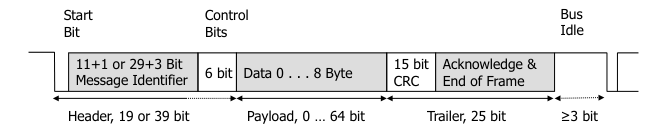
\includegraphics[width=0.4\textwidth]{./images/can_data_format.png}
  \caption{Formato dei dati CAN}
  \label{fig:can_data_format}
\end{figure}

\textbf{CSMA/CR con arbitrato bit per bit}
\begin{itemize}
    \item Evita collisioni tramite l'accesso al bus controllato dalla priorità.
    \item Ogni messaggio contiene un identificativo corrispondente alla sua priorità.
    \item L'identificativo codifica "0" dominante e "1" recessivo: la trasmissione simultanea di "0" e "1" produce un "0".
    \item Riempimento dei bit: dopo 5 bit identici, viene inserito un bit di riempimento invertito (ignorato dal ricevitore).
    \item Quando nessuna stazione sta trasmettendo, il bus legge "1" (stato recessivo).
    \item La sincronizzazione avviene a livello di bit, rilevando il bit di inizio della stazione trasmittente.
    \item Attendere la fine della trasmissione corrente.
    \item Attendere 6 bit recessivi consecutivi.
    \item Inviare l'identificativo (mentre si ascolta il bus).
    \item Osservare una discrepanza tra il livello di segnale trasmesso e rilevato.
    \item Questo indica che si è verificata una collisione con un messaggio di priorità superiore.
    \item Ritirarsi dall'accesso al bus e riprovare in seguito.
    \item Realizzazione di uno schema di priorità non pre-emptive.
    \item Garanzie in tempo reale per i messaggi con priorità più alta, ad esempio, messaggi con il più lungo prefisso "0".
\end{itemize}



Esempio di arbitrato bit per bit(\autoref{fig:can_bitwise_example}):
\begin{figure}[!ht]
  \centering
  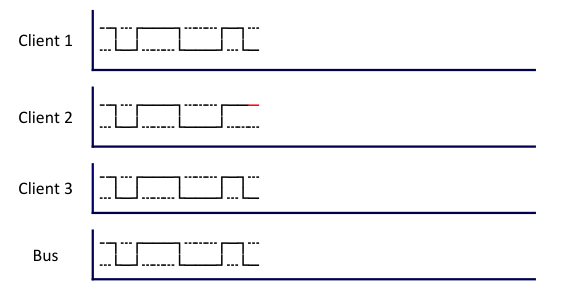
\includegraphics[width=0.4\textwidth]{./images/can_bitwise_example.png}
  \caption{Esempio di arbitrato bit per bit}
  \label{fig:can_bitwise_example}
\end{figure}

In questo caso il client 2 si rende conto che c'è un problema e fa \textbf{back off} lasciando libero il bus.
\begin{figure}[!ht]
  \centering
  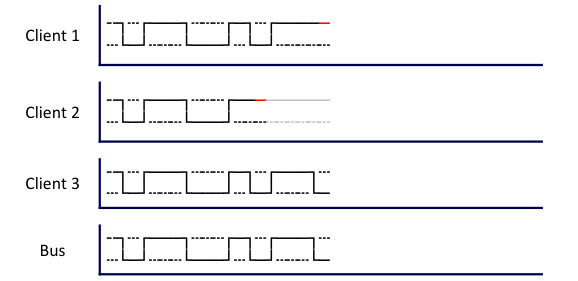
\includegraphics[width=0.4\textwidth]{./images/can_bitwise_example_pt2.png}
  \caption{Esempio di arbitrato bit per bit}
  \label{fig:can_bitwise_example_pt2}
\end{figure}

In \autoref{fig:can_bitwise_example_pt2} il client 1 si rende conto del bus impegnato da una comunicazione con priorità maggiore e fa \textbf{backoff} che porta a mantenere sul bus la comunicazione con priorità maggiore(client 3) e poi segue la trasmissione del dato che il client 3 deve trasmettere.




\subsubsection{TTCAN(Time triggered CAN)}
un problema del CAN è quello della temporizzazione e del mantenimento dei clock fra i client.

Per risolvere questo problema è stato creato il TTCAN, che ha un nodo dedicato che prende il nome di \textbf{time master} è che periodicamente manda un segnale \textbf{basic cycles} a tutti i nodi.

Con \textbf{basic cycle} si intende un numero definito di slot occupabili che vengono popolati da una fase di organizzazione per priorità all'inizio della stessa.


CAN non si può usare per real time communications.

\subsubsection{Message Filtering}

I messaggi vengono accettati in base al loro identificativo mediante l'uso di due registri:
\begin{figure}[!ht]
  \centering
  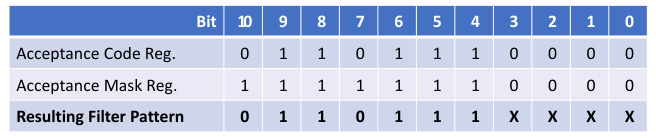
\includegraphics[width=0.4\textwidth]{./images/can_filte.png}
  \caption{Registri di filtraggio CAN}
  \label{fig:can_filter}
\end{figure}


\subsubsection{Data Format}

Il formato di dati segue:
\begin{itemize}
  \item NRZ
  \item bit stuffing
  \item il frame inizia con un bit significativo(0)
  \item il message idenfier è 11 Bit(CAN 2.0A) oppure adesso 29Bit (CAN 2.0B)
  \item Bit di controllo idenficano il tipo di messaggio e la lunghezza
  \item payload: massimo 8 Byte, trasmesso a $500kBit/s$
  \item i dati interessanti del frame sono pochi e quindi il data rate effettivo è $30kBit/s$
\end{itemize}

\begin{figure}[!ht]
  \centering
  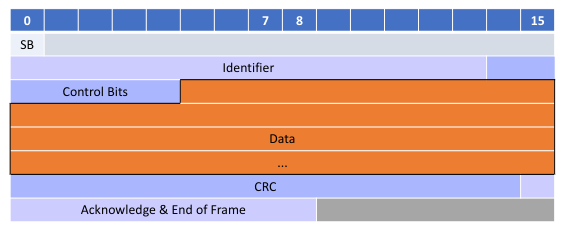
\includegraphics[width=0.4\textwidth]{./images/can_data_format_2.png}
  \caption{Data format}
  \label{fig:can_format_2}
\end{figure}



\subsubsection{Error detection LOW LEVEL}
\begin{itemize}
    \item Il mittente verifica la presenza di livelli di segnale inattesi sul bus.
    \item Tutti i nodi monitorano i messaggi sul bus.
    \item Tutti i nodi verificano la conformità del protocollo dei messaggi.
    \item Tutti i nodi controllano il riempimento dei bit.
    \item Il ricevitore verifica il CRC.
    \item Se uno qualsiasi dei nodi rileva un errore, trasmette un segnale di errore.
      (6 bit dominanti senza bit stuffing)
    \item Tutti i nodi rilevano il segnale di errore e scartano il messaggio.
\end{itemize}





\subsubsection{Error detection HIGH LEVEL}


\begin{itemize}
    \item Il mittente verifica la ricezione di un riconoscimento.
      (Il ricevitore trasmette un bit dominante "0" durante il campo di ACK del messaggio ricevuto)
    \item Ripetizione automatica delle trasmissioni fallite.
    % \item Se il controller si rende conto di causare troppi errori:
    %     \begin{itemize}
    %         \item Sospendere temporaneamente l'accesso al bus.
    %     \end{itemize}
    \item Probabilità residua di fallimento circa $10^{-11}$.
\end{itemize}




\subsubsection{Transoport Layer}
Utile alla gestione del flusso, e gestioen dei frammenti di un singolo messaggio divisi in più data frames.

I due protocolli sono:
\begin{itemize}
  \item ISO-TP
  \item TP 2.0
\end{itemize}

\subsubsection{ISO-TP}
\begin{figure}[!ht]
  \centering
  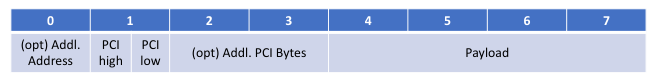
\includegraphics[width=0.4\textwidth]{./images/can_iso_tp.png}
  \caption{ISO-TP}
  \label{fig:can_iso_tp}
\end{figure}


L'\textbf{HEADER} introduce un byte opzionale per l'adressing e da 1 a 3 byte \textbf{PCI}(Protocol Control Information) che identificano il tipo di messaggio e byte specifici al messaggio.


\textbf{Single-frame} è identificato da 1 byte PCI, l'high-niggle(4bit) è 0, e il low-nibble identifica i bytes in payload, non è possibile fare controllo di flusso.

\textbf{First-frame}: identificato da 2 bytes PCI, high-nibble è 1 e low-nibble con aggiunta di 1 byte definisce la dimensione del payload.

Dopo il primo frame il sender aspetta il \textbf{flow control frame}.

\textbf{Consecutive-frame}: 1 byte PCI, high nibble è 2, low nibble è un numero d isequenza \textbf{SN} che parte da 1

\textbf{Flow control-frame}: 3 bytes pci, high nibble è 3 e low nibble specifica lo stato del flusso \textbf{FS}
\begin{itemize}
  \item FS 1: clear to send
  \item FS 2: wait
\end{itemize}

Il byte 2 specifica la block size BS e il byte 3 indica ST(separation time).




\subsubsection{TP 2.0}
Protocollo simile a TCP:
\begin{itemize}
  \item connection oriented
  \item comunicazione basata su canali
  \item specifica fasi di: setup, configurazione, trasmissione e chisura
  \item ogni ECU ha un'indirizzo
\end{itemize}




\textbf{Broadcast}
\begin{itemize}
  \item ripetizione per 5 volte per evitare perdita
  \item Byte 0: adress of desctination ECU
  \item Byte 1: operation code(broadcast response or request)
  \item Byte 2, 3, 4: Service ID(SID) 
  \item Byte 5, 6: Response (si alterna 0x5555 e 0xAAAA per dire che non si vuole aspettare risposta)
\end{itemize}



\textbf{Channel setup}
\begin{itemize}
  \item Byte 0: adress destination ECU
  \item Byte 1: Operation code(Channel request, positive response e negative response)
  \item Byte 2, 3: RX ID(presente se validity nibble di Byte 3 è 0 altrimenti non settato)
  \item Byte 4, 5: TX ID(presente se validity nibble di Byte 5 è 0 altrimenti non settato)
  \item Byte 6: application type
\end{itemize}





\textbf{Impostazione dei parametri del canale}
Nel contesto del protocollo TP 2.0 del Bus CAN, sono previste operazioni di impostazione dei parametri del canale. Il Byte 0 indica l'opcode, che può essere 0xA0 per la "Richiesta di configurazione del canale" (parametri per il canale verso l'iniziatore) o 0xA1 per la "Risposta di configurazione del canale" (parametri per il canale inverso). Il Byte 1 specifica la dimensione del blocco, ovvero il numero di messaggi CAN che il mittente deve attendere prima di ricevere un ACK. I Byte 2, 3, 4 e 5 definiscono i parametri di temporizzazione, ad esempio il tempo minimo tra due messaggi CAN.

\textbf{Gestione generale e chiusura del canale}
Nel contesto del protocollo TP 2.0 del Bus CAN, sono previste operazioni di gestione generale e chiusura del canale. Il Byte 0 specifica l'opcode, che può essere 0xA3 per il "Test" (che riceverà una risposta con la "Risposta di configurazione della connessione"), 0xA4 per il "Break" (in cui il ricevitore scarta i dati dall'ultimo ACK in poi) o 0xA5 per la "Disconnessione" (in cui il ricevitore risponde con una disconnessione).

\textbf{Trasmissione di dati tramite canali}
Nel protocollo TP 2.0 del Bus CAN, la trasmissione di dati avviene tramite canali. Il Byte 0, con il nibble alto, specifica l'opcode. Quando il bit più significativo (MSB) è 0, indica un payload. Quando /AR è 0, indica che il mittente sta ora aspettando un ACK. Quando EOM è 1, indica che si tratta dell'ultimo messaggio di un blocco. Quando il MSB è 1, il messaggio è solo un ACK, senza payload. Quando RS è 1, il canale è pronto per il prossimo messaggio, è un meccanismo di controllo del flusso. Il nibble basso del Byte 0 rappresenta il numero di sequenza. I Byte da 1 a 7 contengono il payload.





\subsubsection{CAN - main takeaways}

\begin{itemize}
  \item BUS standard nei veicoli
  \item message oriented
  \item CSMA con bitwise arbitration
  \item error detection
  \item Transport layer: ISO-TP VS TP 2.0
\end{itemize}

\subsection{LIN: Local Interconnect Network} % (fold)
\label{sub:LIN: Local Interconnect Network}

Il goal principale del LIN bus è quello di essere poco costoso di low speed can, la specfica riguarda
lo strato fisoc e data link layer.

LIN è simile a K-Line e sfrutta il concetto di master-slave, il nodo master solitamente
fa parte di un bus CAN, infatti il lin bus prende il nome di sub bus solitamente.

Il LIN bus è formato di un solo filo e offre una comunicazione bidirezionale fino a velocità
di $20kBit/s$.

La trasmissione dei bit è compatibile con UART(1 start bit basso, 8 data bit e 1 stop bit alto) e la comunicazione è del tipo message oriented, quindi non ci sono indirizzi.


L'errore è percepito mediante l'ascolto dell'energia del canale di comunicazione, non è presente una metodo di correzione dell'errore.

I messaggi sono scanditi da cicli temporali definiti dal master.

I segnali inviati dal master sono:
\begin{enumerate}
  \item sync break: 13 bit bassi e 1 bit alto
  \item sync byte: 0x55(01010101)
  \item LIN Identifier: 6 bit(I0 fino a I5) + 2 bit di parity
    \begin{itemize}
      \item 0x00 fino a 0x3b sono tipi di dati definit dall'applicazione
      \item 0x3c fino a 0x3d sono messaggi per la diagnosi
      \item 0x3e è un messaggio definito dall'applciazione
      \item 0x3f è un messaggio riservato
      \item i bit di parity sono codficati come % TODO: finire di scrivere la parity a pagina 90 
    \end{itemize}
\end{enumerate}



I segnali inviati dallo slave sono risposte con 8 byte di dati, con codifica LSB first(Least Significant Bit) prende anche il nome di \textbf{Little Endian}.

La lunghezza è identificata dal'identificatore LIN.

I frame di dati finiscono con il checksum che è costruito come somma di tutti i bytes e dei loro riporti.


\subsubsection{Types of requests} % (fold)
\label{sec:Types of requests}

Gli \textbf{unconditionl frame} sono i frame più semplici, progettati per \textit{pooling periodico} e sono uno slave risponde.
Un esempio è: "la porta davanti a destra ha cambiato stato?".


Gli \textbf{event triggered frame} viene effettuato il \textbf{pooling} da tanti slaves, spesso questa richiesta viene avviata dal can.
Può portare a collissione che il master riconosce dai dati corrotti e richiede dati individualemnte agli slaves.

Gli \textbf{sporadic frame} inviato dal master solo quando necessario


Un esempio di schedule table è:
\begin{table}[!ht]
  \caption{Schedule table}\label{tab:schedule table}
  \begin{center}
    \begin{tabular}[c]{c c c}
      \hline
      1 & unconditionl & ac \\
      2 & unconditionl & rain sensor \\
      3 & unconditionl & tire pressure \\
      4 & event triggered & door status \\
      5 & sporaic & temperature \\
      \hline
    \end{tabular}
  \end{center}
\end{table}





% subsubsection Types of requests (end)

Per fare la diagnosi esterna e interrogare il bus lin si procede in due modi:
\begin{itemize}
  \item si interroga il master collegato al can protocol che risponde impersonando i vari nodi della sua sotto rete
  \item si interroga direttamente il nodo lin e quindi il master deve fare tunnellign dei dati(schefezza ma più sofisticato)
\end{itemize}

\subsubsection{Main takeaways} % (fold)
\label{sec:Main takeaways}
% TODO: aggiungee da pagina 97 e 98

% subsubsection Main takeaways (end)


% subsection LIN: Local Interconnect Network (end)


\subsection{FlexRay} % (fold)
\label{sub:FlexRay}

Le motivazioni per lo sviluppo di flexray sono:
\begin{itemize}
  \item tutto fatto by wire (X-By-Wire)
  \item can bus non ha ridondanza ed è facile che fallisca
  \item can bus è lento
  \item can bus non è deterministico
\end{itemize}

Le soluzioni principali sono state introdotte da OEM(Original Equipment Manufacturer) e le proposte sono state TTCAN, TTP/TTA ecc.

Alla fine BMW, VW, Bosch e altri hanno fatto un consorzio e realizzato un nuovo bus chiamato felxray.

La topologia di rete è:

\begin{figure}[!ht]
  \begin{adjustbox}{width=0.5\columnwidth, center}
    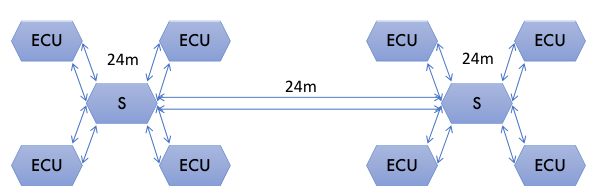
\includegraphics{images/flexray.png}
  \end{adjustbox}
  \caption{FlexRay network}
  \label{fig:flexray_network}
\end{figure}

si usano solitamente due canali per comunicare cosi da avere due comunicazioni parallere la $10 MBit/s$ che si sommano e danno $20 MBit/s$.


La trasmissione necessita di sincronizzazione tra sender e receiver.

Non viene utilizzato il bit stuffing per mantenere la lunghezza dei dati deterministica.


% TODO: stoppato a pagina 102
% TODO: ripreso a pagina 141



% subsection FlexRay (end)



\end{document}





% WARN: per le immagini uso questo metodo

% \begin{figure}[!ht]
%   \begin{adjustbox}{width=0.5\columnwidth, center}
%     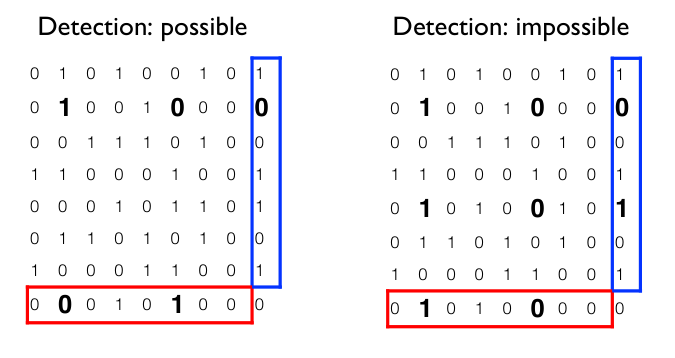
\includegraphics{images/parity_block.png}
%     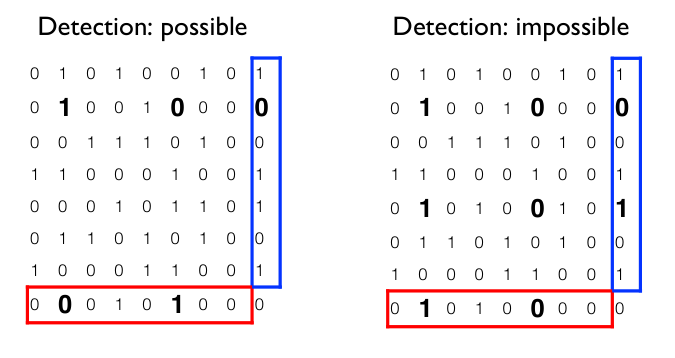
\includegraphics{./images/parity_block.png}
%   \end{adjustbox}
%     \caption{Parity block}
%     \label{fig:parity_block}
% \end{figure}
